\documentclass{beamer}

\usepackage{subfigure}
\usepackage[english]{babel}
\usepackage[latin1]{inputenc}
\usepackage{times}
\usepackage[T1]{fontenc} 
\usepackage{color}

\usepackage{algorithm}
\usepackage{algorithmicx}
\usepackage[noend]{algpseudocode}

\usepackage{minted}

\usetheme[secheader]{Boadilla}
\usefonttheme[onlylarge]{structurebold}
\setbeamerfont*{frametitle}{size=\normalsize,series=\bfseries}
\setbeamertemplate{navigation symbols}{}
\setbeamertemplate{mini frames}[box]
\setbeamertemplate{sections/subsections in toc}[square]
\setbeamertemplate{blocks}[rounded][shadow=true]
\setbeamertemplate{bibliography item}[text]

\setbeamercolor{lightorange}{fg=black,bg=orange!40}
\setbeamercolor{lightblue}{fg=black,bg=blue!30}

\newenvironment{colorblock}[2]
{\setbeamercolor{item}{fg=#1,bg=#1}\begin{beamerboxesrounded}[upper=#1,lower=#2,shadow=true]}
  {\end{beamerboxesrounded}}



% Setup TikZ

\usepackage{tikz}
\usetikzlibrary{arrows}
\tikzstyle{block}=[draw opacity=0.7,line width=1.4cm]


%%%%%%%%%%%%%%%%%%%%%%%%%%%%%%%%%%%%%
%%%%%%%%%%%%%%%%%%%%%%%%%%%%%%%%%%%%%
%%%%%%%%%%%%%%%%%%%%%%%%%%%%%%%%%%%%%

\newtheorem{observation}[theorem]{Observation} 

%%%%%%%%%%%%%%%%%%%%%%%%%%%%%%%%%%%%%
%%%%%%%%%%%%%%%%%%%%%%%%%%%%%%%%%%%%%
%%%%%%%%%%%%%%%%%%%%%%%%%%%%%%%%%%%%%

\title{Spark SQL}
\subtitle{Architecture and Data Structures}
\author{Pietro Michiardi}
\institute{Eurecom}
\date


\begin{document}

\begin{frame}
  \titlepage
\end{frame}

%%%%%%%%%%%%%%%%%%%%%%%%%%%%%%%%%%%%%%%%%%%%%%%%%%%%%%%%%%
\section{Sources and Acks}

\begin{frame}
  \begin{itemize}
    \item M. Aembrust, et. al., ``Spark SQL: Relational Data Processing in Spark'', in Proc. of ACM Sigmod 2015

    \item[]

    \item Lookup for slides on SlideShare, and videos around the web!
  \end{itemize}
\end{frame}

%%%%%%%%%%%%%%%%%%%%%%%%%%%%%%%%%%%%%%%%%%%%%%%%%%%%%%%%%%


%%%%%%%%%%%%%%%%%%%%%%%%%%%%%%%%%%%%%%%%%%%%%%%%%%%%%%%%%%
\section{Introduction}

\begin{frame}
 \begin{colorblock}{blue}{lightblue}{ }
  \begin{center}
    \Huge \textbf{\texttt{Introduction}}
  \end{center}
  \end{colorblock}
\end{frame}

%%%%%%%%%%%%%%%%%%%%%%%%%%%%%%%%%%%%%%%%%%%%%%%%%%%%%%%%%%
\frame {\frametitle{Introduction}
%%%%%%%%%%%%%%%%%%%%%%%%%%%%%%%%%%%%%%%%%%%%%%%%%%%%%%%%%%
\begin{itemize}
  \item {\bf High-level programming language: SQL}
  \begin{itemize}
    \item Expressiveness, succinctness
    \item Enables compatibility with existing tools, e.g. BI using JDBC
    \item Large pool of engineers proficient in SQL
  \end{itemize}

  \item[]

  \item {\bf Project goals}
  \begin{itemize}
    \item Write less code
    \item Read less data
    \item Let the optimizer do the hard work
  \end{itemize}

  \item[]

  \item {\bf Design philosophy}
  \begin{itemize}
    \item SparkSQL is a Library
    \item Uses the SparkContext to interact with Spark
  \end{itemize}
\end{itemize}
}

%%%%%%%%%%%%%%%%%%%%%%%%%%%%%%%%%%%%%%%%%%%%%%%%%%%%%%%%%%
\frame {\frametitle{Challenges}
%%%%%%%%%%%%%%%%%%%%%%%%%%%%%%%%%%%%%%%%%%%%%%%%%%%%%%%%%%
\begin{itemize}
  \item {\bf Variety of data source formats}
  \begin{itemize}
    \item ETL workloads often involve working with various kinds of data
    \item[$\to$] DataSource API
  \end{itemize}

  \item[]
  
  \item {\bf SQL implementation}
  \begin{itemize}
    \item Extensibility, e.g. to cover SQL standard
    \item[$\to$] DataFrame API

    \item[]
    
    \item Efficiency
    \item[$\to$] Catalyst optimizer
  \end{itemize}

\end{itemize}
}

%%%%%%%%%%%%%%%%%%%%%%%%%%%%%%%%%%%%%%%%%%%%%%%%%%%%%%%%%%
\frame {\frametitle{Outline}
%%%%%%%%%%%%%%%%%%%%%%%%%%%%%%%%%%%%%%%%%%%%%%%%%%%%%%%%%%
\begin{itemize}
  \item {\bf Spark and SparkSQL data structures}

  \item[]
  
  \item {\bf Functional architecture, with a RDBMS flavor}
  
  \item[]
  
  \item {\bf Performance}
\end{itemize}
}

%%%%%%%%%%%%%%%%%%%%%%%%%%%%%%%%%%%%%%%%%%%%%%%%%%%%%%%%%%

%%%%%%%%%%%%%%%%%%%%%%%%%%%%%%%%%%%%%%%%%%%%%%%%%%%%%%%%%%
\section{Data Structures}

\begin{frame}
 \begin{colorblock}{blue}{lightblue}{ }
  \begin{center}
    \Huge \textbf{\texttt{Data Representation}}
  \end{center}
  \end{colorblock}
\end{frame}

%%%%%%%%%%%%%%%%%%%%%%%%%%%%%%%%%%%%%%%%%%%%%%%%%%%%%%%%%%
\frame {\frametitle{DataSource API}
%%%%%%%%%%%%%%%%%%%%%%%%%%%%%%%%%%%%%%%%%%%%%%%%%%%%%%%%%%
\begin{itemize}
  \item {\bf Read and write with a variety of formats}
\end{itemize}

\begin{figure}[htbp]
	\centering
	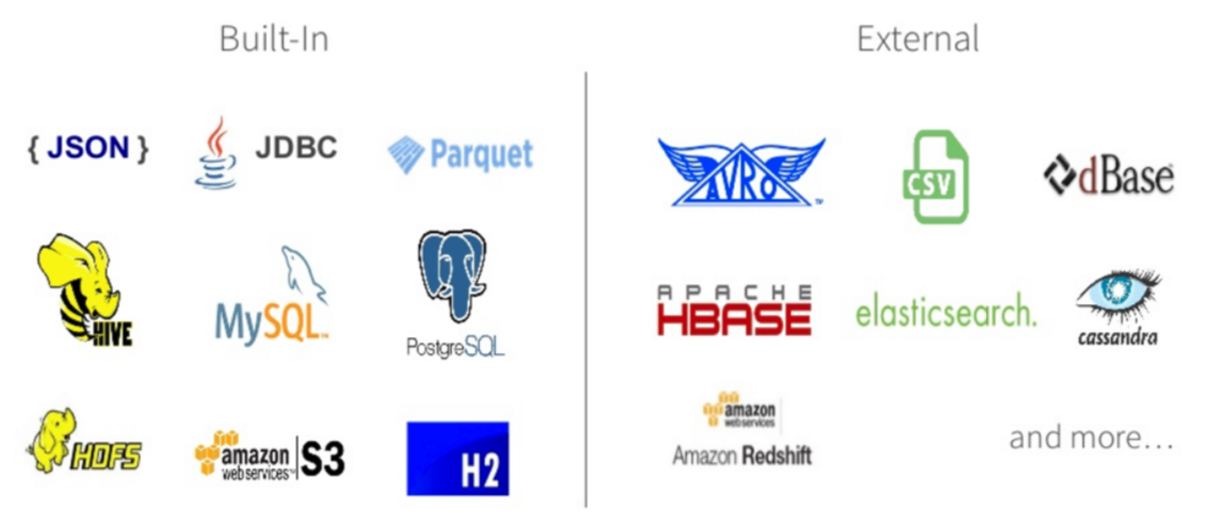
\includegraphics[width=0.95\textwidth]{figures/dataformats}
\end{figure}
}


%%%%%%%%%%%%%%%%%%%%%%%%%%%%%%%%%%%%%%%%%%%%%%%%%%%%%%%%%%
\begin{frame}[fragile=singleslide]{DataSource API}
%%%%%%%%%%%%%%%%%%%%%%%%%%%%%%%%%%%%%%%%%%%%%%%%%%%%%%%%%%
\begin{itemize}
	\item Unified interface to reading data
	\item {\color{red}read} function creates new I/O builders
	\item {\color{green}load} function creates new I/O builders
\end{itemize}

\vspace{20pt}

\begin{minted}{python}
df = sqlContext.read \
  .format(''json'') \
  .option(''samplingRatio'', ''0.1'') \
  .load(''data.json'')
\end{minted}

\end{frame}

%%%%%%%%%%%%%%%%%%%%%%%%%%%%%%%%%%%%%%%%%%%%%%%%%%%%%%%%%%
\begin{frame}[fragile=singleslide]{DataSource API}
%%%%%%%%%%%%%%%%%%%%%%%%%%%%%%%%%%%%%%%%%%%%%%%%%%%%%%%%%%
\begin{itemize}
	\item Unified interface to writing data
	\item {\color{red}Write} function creates new I/O builders
	\item {\color{green}save} function creates new I/O builders
\end{itemize}

\vspace{20pt}

\begin{minted}{python}
df.write \
  .format(''parquet'') \
  .mode(''append'') \
  .partitionBy(''year'') \
  .saveAsTable(''myData'')
\end{minted}

\end{frame}

%%%%%%%%%%%%%%%%%%%%%%%%%%%%%%%%%%%%%%%%%%%%%%%%%%%%%%%%%%
\frame {\frametitle{DataSource API}
%%%%%%%%%%%%%%%%%%%%%%%%%%%%%%%%%%%%%%%%%%%%%%%%%%%%%%%%%%
\begin{itemize}
	\item {\bf Builder methods}
	\begin{itemize}
		\item Specify data format
		\item Define data partitioning
		\item Handle existing data
		\item ... and much more
	\end{itemize}

\end{itemize}
}

%%%%%%%%%%%%%%%%%%%%%%%%%%%%%%%%%%%%%%%%%%%%%%%%%%%%%%%%%%
\frame {\frametitle{DataFrame}
%%%%%%%%%%%%%%%%%%%%%%%%%%%%%%%%%%%%%%%%%%%%%%%%%%%%%%%%%%
\begin{itemize}
	\item {\bf Schema to the rescue}
	\begin{itemize}
		\item A distributed collection of rows organized into named columns
		\item Schema inference can be automatic
	\end{itemize}

	\item[]
	
	\item {\bf Structured data}
	\begin{itemize}
		\item An abstraction for selecting, filtering, aggregating and plotting structured data
	\end{itemize}
	
\end{itemize}
}

%%%%%%%%%%%%%%%%%%%%%%%%%%%%%%%%%%%%%%%%%%%%%%%%%%%%%%%%%%
\frame {\frametitle{DataFrame}
%%%%%%%%%%%%%%%%%%%%%%%%%%%%%%%%%%%%%%%%%%%%%%%%%%%%%%%%%%
\begin{itemize}
	\item {\bf General idea borrowed from Python Pandas}
	\begin{itemize}
		\item Tabular data with an API
		\item Math, stats, algebra, ...
	\end{itemize}

	\item[]

	\item {\bf Relation to a low-level RDD}
	\begin{itemize}
		\item Introduces structure to the data
		\item Specific relational operators
		\begin{itemize}
			\item Select required columns
			\item Join different data sources
			\item Aggregation operations
			\item Filtering
		\end{itemize}
	\end{itemize}
\end{itemize}
}

%%%%%%%%%%%%%%%%%%%%%%%%%%%%%%%%%%%%%%%%%%%%%%%%%%%%%%%%%%
\begin{frame}[fragile=singleslide]{DataFrame API}
%%%%%%%%%%%%%%%%%%%%%%%%%%%%%%%%%%%%%%%%%%%%%%%%%%%%%%%%%%
\begin{itemize}
	\item Example using RDDs
\end{itemize}

\begin{minted}[fontsize=\footnotesize]{python}
data = sc.textFile(...).split('' '')
data.map(lambda x: (x[0], [int(x[1]), 1])) \
  .reduceByKey(lambda x, y: [x[0] + y[0], x[1] + y[1]]) \
  .map(lambda x: [x[0], x[1][0] / x[1][1]]) \
  .collect()
\end{minted}

\end{frame}

%%%%%%%%%%%%%%%%%%%%%%%%%%%%%%%%%%%%%%%%%%%%%%%%%%%%%%%%%%
\begin{frame}[fragile=singleslide]{DataFrame API}
%%%%%%%%%%%%%%%%%%%%%%%%%%%%%%%%%%%%%%%%%%%%%%%%%%%%%%%%%%
\begin{itemize}
	\item Example using SQL
\end{itemize}

\begin{minted}{sql}
SELECT name, avg(age)
FROM people
GROUP BY name
\end{minted}

\end{frame}

%%%%%%%%%%%%%%%%%%%%%%%%%%%%%%%%%%%%%%%%%%%%%%%%%%%%%%%%%%
\begin{frame}[fragile=singleslide]{DataFrame API}
%%%%%%%%%%%%%%%%%%%%%%%%%%%%%%%%%%%%%%%%%%%%%%%%%%%%%%%%%%
\begin{itemize}
	\item Example using DataFrames
\end{itemize}

\begin{minted}{python}
sqlContext.table(''people'') \
  .groupBy(''name'') \
  .agg(''name'', avg(''age'')) \
  .collect()
\end{minted}

\end{frame}

%%%%%%%%%%%%%%%%%%%%%%%%%%%%%%%%%%%%%%%%%%%%%%%%%%%%%%%%%%

%%%%%%%%%%%%%%%%%%%%%%%%%%%%%%%%%%%%%%%%%%%%%%%%%%%%%%%%%%
\section{Architecture}

\begin{frame}
 \begin{colorblock}{blue}{lightblue}{ }
  \begin{center}
    \Huge \textbf{\texttt{Architecture}}
  \end{center}
  \end{colorblock}
\end{frame}

%%%%%%%%%%%%%%%%%%%%%%%%%%%%%%%%%%%%%%%%%%%%%%%%%%%%%%%%%%
\frame {\frametitle{Background and roadmap}
%%%%%%%%%%%%%%%%%%%%%%%%%%%%%%%%%%%%%%%%%%%%%%%%%%%%%%%%%%
\begin{itemize}
  \item {\bf Reminiscent of traditional database systems}
  \begin{itemize}
  	\item Abstract representation of SQL expressions
  	\item Optimizations for efficiency and performance
  	\item Sophisticated cost model
  \end{itemize}

  \item[]

  \item {\bf Focus on optimizations}
  \begin{itemize}
  	\item Logical plan
  	\item Physical plan
  	\item Cost-based vs. Rule-based
  \end{itemize}
\end{itemize}
}

%%%%%%%%%%%%%%%%%%%%%%%%%%%%%%%%%%%%%%%%%%%%%%%%%%%%%%%%%%
\frame {\frametitle{Global view}
%%%%%%%%%%%%%%%%%%%%%%%%%%%%%%%%%%%%%%%%%%%%%%%%%%%%%%%%%%
\begin{figure}[htbp]
	\centering
	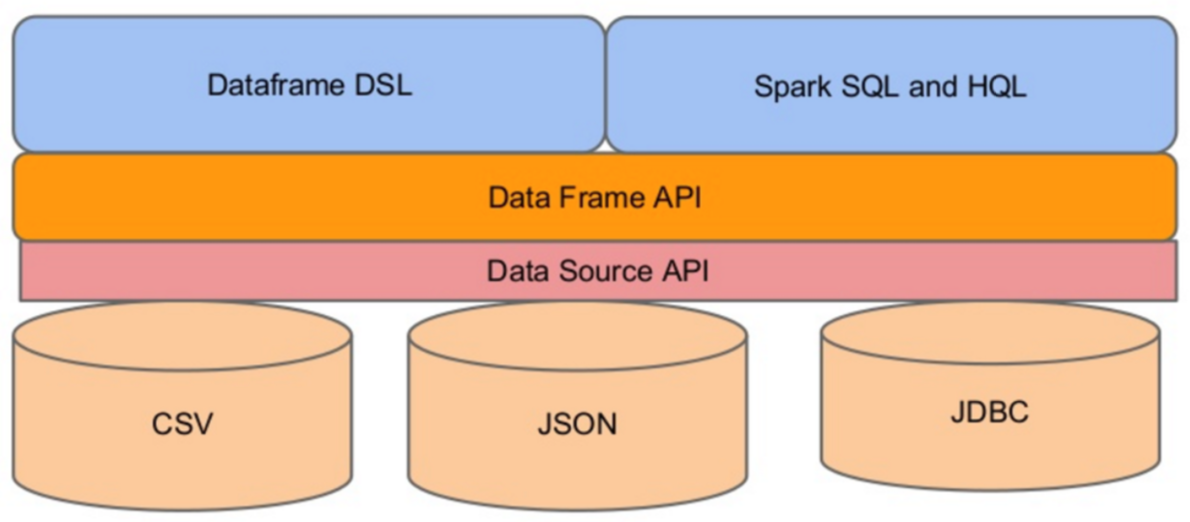
\includegraphics[width=0.95\textwidth]{figures/overview}
\end{figure}
}

%%%%%%%%%%%%%%%%%%%%%%%%%%%%%%%%%%%%%%%%%%%%%%%%%%%%%%%%%%
\frame {\frametitle{SparkSQLContext}
%%%%%%%%%%%%%%%%%%%%%%%%%%%%%%%%%%%%%%%%%%%%%%%%%%%%%%%%%%
\begin{figure}[htbp]
	\centering
	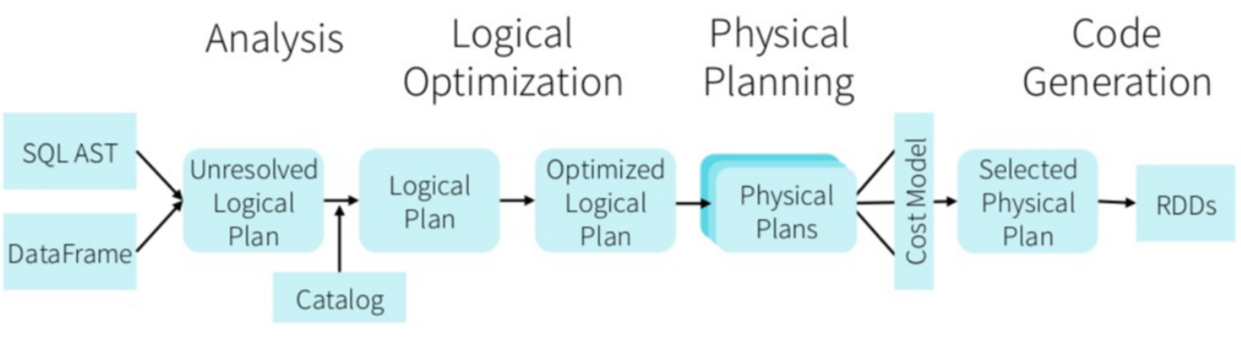
\includegraphics[width=0.95\textwidth]{figures/architecture}
\end{figure}
}

%%%%%%%%%%%%%%%%%%%%%%%%%%%%%%%%%%%%%%%%%%%%%%%%%%%%%%%%%%
\frame {\frametitle{Catalyst optimizer}
%%%%%%%%%%%%%%%%%%%%%%%%%%%%%%%%%%%%%%%%%%%%%%%%%%%%%%%%%%
\begin{itemize}
	\item {\bf Overall goals}
	\begin{itemize}
		\item Optimize logical plan
		\item Convert logical to physical plan
		\item Optimize physical plan
		\item Code generation
	\end{itemize}

	\item[]

	\item {\bf Explot \texttt{scala} language features}
	\begin{itemize}
		\item \texttt{Quasiquotes}
		\item Abstract syntax tree
		\item Tree manipulation library
		\item Optimizations rules implemented as tree transformations
	\end{itemize}
\end{itemize}
}

%%%%%%%%%%%%%%%%%%%%%%%%%%%%%%%%%%%%%%%%%%%%%%%%%%%%%%%%%%
\begin{frame}[fragile=singleslide]{Example query}
%%%%%%%%%%%%%%%%%%%%%%%%%%%%%%%%%%%%%%%%%%%%%%%%%%%%%%%%%%
\begin{columns}

\begin{column}{0.5\textwidth}
\begin{minted}{sql}
SELECT name
FROM (
	SELECT id, name
	FROM People) p
WHERE p.id = 1
\end{minted}
\end{column}

\begin{column}{0.5\textwidth}
   	\begin{center}
     		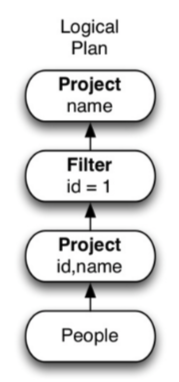
\includegraphics[width=0.5\textwidth]{figures/ex-p1}
   	\end{center}
\end{column}
\end{columns}
\end{frame}

%%%%%%%%%%%%%%%%%%%%%%%%%%%%%%%%%%%%%%%%%%%%%%%%%%%%%%%%%%
\begin{frame}[fragile=singleslide]{Example query}
%%%%%%%%%%%%%%%%%%%%%%%%%%%%%%%%%%%%%%%%%%%%%%%%%%%%%%%%%%
\begin{columns}

\begin{column}{0.5\textwidth}
Native query planning
\begin{minted}{sql}
SELECT name
FROM (
	SELECT id, name
	FROM People) p
WHERE p.id = 1
\end{minted}
\end{column}

\begin{column}{0.5\textwidth}
   	\begin{center}
     		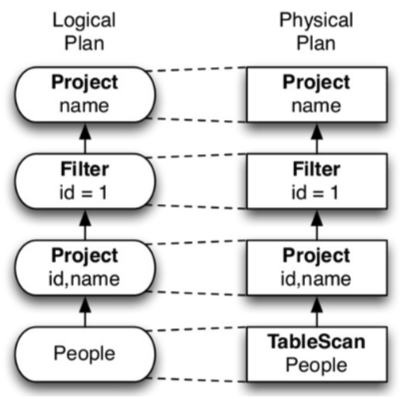
\includegraphics[scale=0.4]{figures/ex-p2}
   	\end{center}
\end{column}
\end{columns}
\end{frame}

%%%%%%%%%%%%%%%%%%%%%%%%%%%%%%%%%%%%%%%%%%%%%%%%%%%%%%%%%%
\begin{frame}[fragile=singleslide]{Example query}
%%%%%%%%%%%%%%%%%%%%%%%%%%%%%%%%%%%%%%%%%%%%%%%%%%%%%%%%%%
\begin{columns}

\begin{column}{0.5\textwidth}
Optimization rules example
\begin{itemize}
	\item Find filters on top of projections
	\item Check that filters can be evaluated without the result of the projection
	\item If yes, switch operators
\end{itemize}
\end{column}

\begin{column}{0.5\textwidth}
   	\begin{center}
     		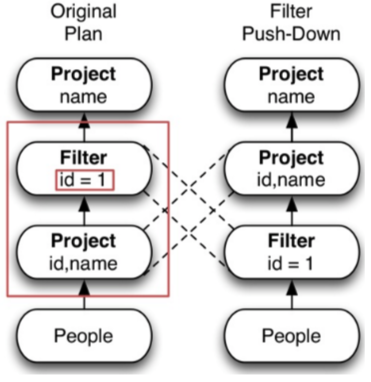
\includegraphics[scale=0.4]{figures/ex-p3}
   	\end{center}
\end{column}
\end{columns}
\end{frame}

%%%%%%%%%%%%%%%%%%%%%%%%%%%%%%%%%%%%%%%%%%%%%%%%%%%%%%%%%%
\begin{frame}[fragile=singleslide]{Example query}
%%%%%%%%%%%%%%%%%%%%%%%%%%%%%%%%%%%%%%%%%%%%%%%%%%%%%%%%%%
\begin{itemize}
	\item Definition of custom rules
\end{itemize}

\begin{figure}[htbp]
	\centering
	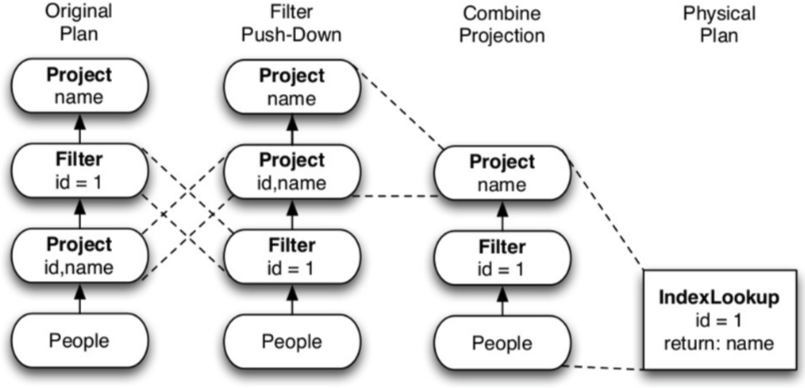
\includegraphics[width=0.95\textwidth]{figures/ex-p4}
\end{figure}

\end{frame}

\frame {\frametitle{Example Optimization Rules}
%%%%%%%%%%%%%%%%%%%%%%%%%%%%%%%%%%%%%%%%%%%%%%%%%%%%%%%%%%
\begin{itemize}
	\item Eliminate subqueries
	\item[]
	\item Constant folding
	\item[]
	\item Simplify filters
	\item[]
	\item PushPredicate through filter
	\item[]
	\item Project collapsing
\end{itemize}
}

%%%%%%%%%%%%%%%%%%%%%%%%%%%%%%%%%%%%%%%%%%%%%%%%%%%%%%%%%%
\frame {\frametitle{Project Tungsten}
%%%%%%%%%%%%%%%%%%%%%%%%%%%%%%%%%%%%%%%%%%%%%%%%%%%%%%%%%%

\begin{itemize}
	\item {\bf Runtime code generation}
	\begin{itemize}
		\item Using code generation to exploit modern compilers and CPUs
	\end{itemize}
	\item[]
	\item {\bf Cache locality}
	\begin{itemize}
		\item Algorithms and data structures to exploit memory hierarchy
	\end{itemize}
	\item[]
	\item {\bf Off-heap memory management}
	\begin{itemize}
		\item Leveraging application semantics to manage memory explicitly and eliminate the overhead of JVM object model and garbage collection
	\end{itemize}
\end{itemize}

}

%%%%%%%%%%%%%%%%%%%%%%%%%%%%%%%%%%%%%%%%%%%%%%%%%%%%%%%%%%
\frame {\frametitle{Advanced features}
%%%%%%%%%%%%%%%%%%%%%%%%%%%%%%%%%%%%%%%%%%%%%%%%%%%%%%%%%%
\begin{itemize}
\item Consider string \texttt{``abcd''}: this is 4 bytes in UTF-8
\end{itemize}

\begin{figure}[htbp]
	\centering
	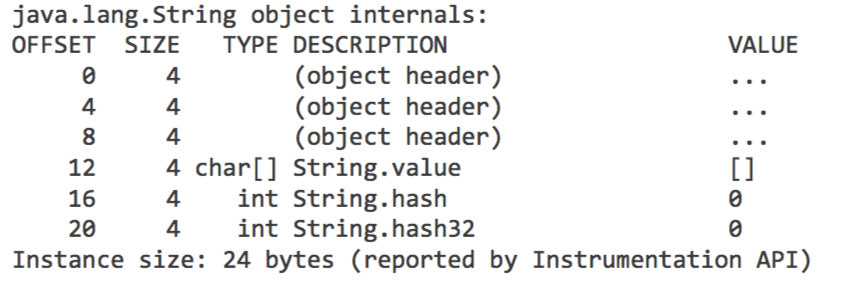
\includegraphics[width=0.95\textwidth]{figures/tungsten}
\end{figure}
}

%%%%%%%%%%%%%%%%%%%%%%%%%%%%%%%%%%%%%%%%%%%%%%%%%%%%%%%%%%

%%%%%%%%%%%%%%%%%%%%%%%%%%%%%%%%%%%%%%%%%%%%%%%%%%%%%%%%%%
\section{Performance}

\begin{frame}
 \begin{colorblock}{blue}{lightblue}{ }
  \begin{center}
    \Huge \textbf{\texttt{Performance}}
  \end{center}
  \end{colorblock}
\end{frame}

%%%%%%%%%%%%%%%%%%%%%%%%%%%%%%%%%%%%%%%%%%%%%%%%%%%%%%%%%%
\frame {\frametitle{Performance comparisons}
%%%%%%%%%%%%%%%%%%%%%%%%%%%%%%%%%%%%%%%%%%%%%%%%%%%%%%%%%%
\begin{figure}[htbp]
	\centering
	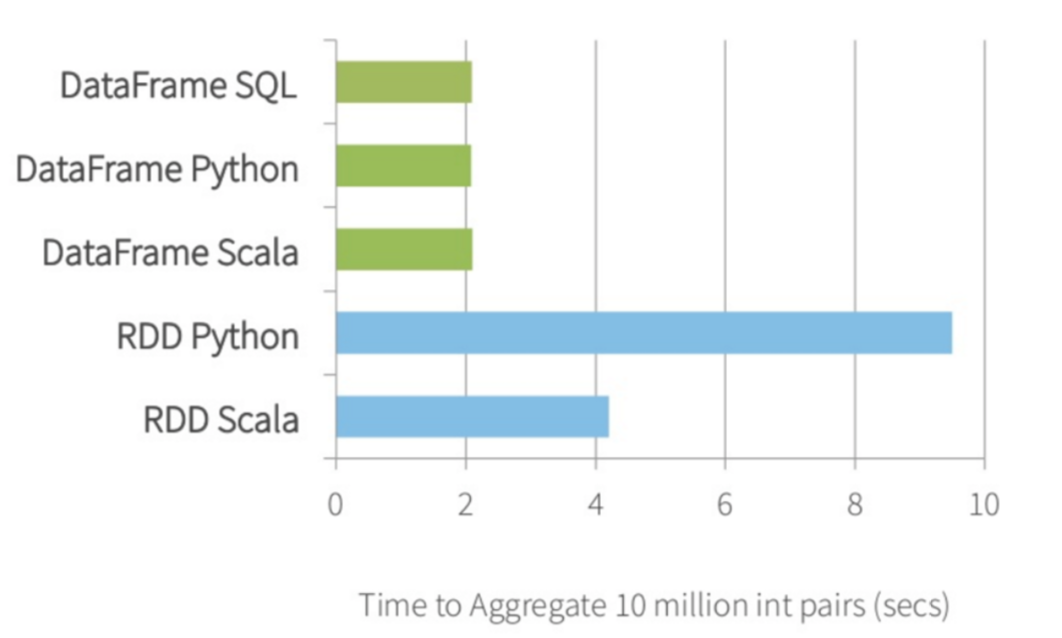
\includegraphics[width=0.95\textwidth]{figures/performance}
\end{figure}
}

%%%%%%%%%%%%%%%%%%%%%%%%%%%%%%%%%%%%%%%%%%%%%%%%%%%%%%%%%%

%%%%%%%%%%%%%%%%%%%%%%%%%%%%%%%%%%%%%%%%%%%%%%%%%%%%%%%%%%
\section{Conclusion}

\begin{frame}
 \begin{colorblock}{blue}{lightblue}{ }
  \begin{center}
    \Huge \textbf{\texttt{Conclusion}}
  \end{center}
  \end{colorblock}
\end{frame}

%%%%%%%%%%%%%%%%%%%%%%%%%%%%%%%%%%%%%%%%%%%%%%%%%%%%%%%%%%
\frame {\frametitle{Conclusion}
%%%%%%%%%%%%%%%%%%%%%%%%%%%%%%%%%%%%%%%%%%%%%%%%%%%%%%%%%%
\begin{itemize}
	\item {\bf Short overview of SparkSQL}
	\begin{itemize}
		\item Borrows many ideas from traditional RDBMs
		\item Standard SQL
		\item Cost-based optimization
		\item Project Tungsten
	\end{itemize}

	\item[]

	\item {\bf Very useful tool for}
	\begin{itemize}
		\item Extract, transform workloads
		\item Simple descriptive statistics
		\item Data exploration, cleaning
	\end{itemize}

	\item[]

	\item {\bf Laboratory on SparkSQL}
	\begin{itemize}
		\item Work on a highly-dimensional dataset
		\item Typical BI queries
	\end{itemize}
\end{itemize}
}

%%%%%%%%%%%%%%%%%%%%%%%%%%%%%%%%%%%%%%%%%%%%%%%%%%%%%%%%%%

%%%%%%%%%%%%%%%%%%%%%%%%%%%%%%%%%%%%%%%%%%%%%%%%%%%%%%%%%%
% \section{References}

% \begin{frame}
%  \begin{colorblock}{blue}{lightblue}{ }
%   \begin{center}
%     \Huge \textbf{\texttt{References}}
%   \end{center}
%   \end{colorblock}
% \end{frame}

% \begin{frame}[allowframebreaks]{References}
% \bibliographystyle{plain} 
% \bibliography{references} 
% \end{frame}
%%%%%%%%%%%%%%%%%%%%%%%%%%%%%%%%%%%%%%%%%%%%%%%%%%%%%%%%%%

\end{document}
